\chapter{Methods and Results}
\label{chap:mar}
To understand \ac{noma} and to create a test-bed to compare future work against I ran simulations of \ac{noma} in MATLAB.

\section{Finding a Suitable Channel Model}
\label{sec:ch}
As a focus of the project is the performance of \ac{noma} in \ac{mmwave} spectrum I first did work to find a suitable \ac{mmwave} Channel model.
Finding such a channel model is important as it has a direct effect on the rate's each \ac{noma} user can achieve.
Throughput, or some derived metric, will be used to determine the success of different \ac{pa} schemes and for comparing \ac{pa} schemes to each other.

\subsection{Friis' Transmission Equation}
It was assumed that a conventional channel model, similar to those used for modern mobile networks, would be unrealistic in it's optimism as the higher frequencies of \acp{mmwave} will weaken faster.
To show this Friis' Transmission Equation for \ac{pl}, \fref{eq:friis}, was taken as a control for comparing other channel models.
A weakness of Friis' Equation is that it assumes free space propagation.
Some channel models use Friis' as a base with some additional loss to account for \ac{nlos} propagation \cite{khan:2011}.

\begin{equation}
	20 \cdot \log_{10} \left( \frac{4 \pi d f}{c} \right)
	\label{eq:friis}
\end{equation}

\par
Where:
\par \indent $d$ is the distance between \ac{ue} and \ac{bs}
\par \indent $f$ is the frequency of the carrier
\par \indent $c$ is the speed of light
\par

\subsection{\acl{ple}}
A common adaptation of the Friis' Equation is the \ac{ple} Equation, shown in \fref{eq:ple}.
\ac{ple} is a common adaptation as the variable exponent is used to counteract the free space \ac{los} assumption of Friis' Equation.

\begin{equation}
	10 \beta \cdot \log_{10} \left( \frac{4 \pi d f}{c} \right)
	\label{eq:ple}
\end{equation}

\par
Where $\beta$ is the exponent and other variables are as above.

\par
I chose to use an exponent value of $3.4$ as it is commonly used for \SI{28}{\giga\hertz} \ac{nlos} channel models \cite{sun:2016,samimi:2016,lee:2018}.
Using figures tuned for \ac{nlos} is sensible as it allows for more realistic simulations.
\ac{los} is very rare in mobile communications, particularly in urban spaces, where \ac{mmwave} is likely to be deployed fist.
I believe that \SI{28}{\giga\hertz} spectrum is a realistic estimate for frequency also.
Though \SI{28}{\giga\hertz} is within \ac{mmwave} spectrum it will be easier to produce hardware for that higher frequencies and it will propagate further than higher frequencies, allowing fewer \acp{bs} to provide coverage.

\subsection{NYU Empirical Model}
\cite{akdeniz:2014} shows an empirical model for \ac{mmwave}, based on results from New York City.
This model describes large scale fading by \fref{eq:nyu}.

\begin{equation}
	PL(d) [\si{\decibel}]= \alpha + 10\beta \cdot \log_{10}(d)
	\label{eq:nyu}
\end{equation}

\par
Once more, choosing values for an \ac{nlos} \SI{28}{\giga\hertz} channel model we get $\alpha = 72.0$ and $\beta = 2.92$.
The justifications for these conditions seen above.

\subsection{Comparing Models}

\Fref{fig:PLcomp} shows a comparison of the \ac{pl} that the above channel models discuss.
The carrier frequency is assumed to be \SI{28}{\giga\hertz}, where applicable values assume \ac{nlos}, and the distances are \SI{88}{\metre} and \SI{330}{\metre} for the \ac{ccu} and \ac{ceu} respectively.

\begin{figure}[htb]
	\centering
	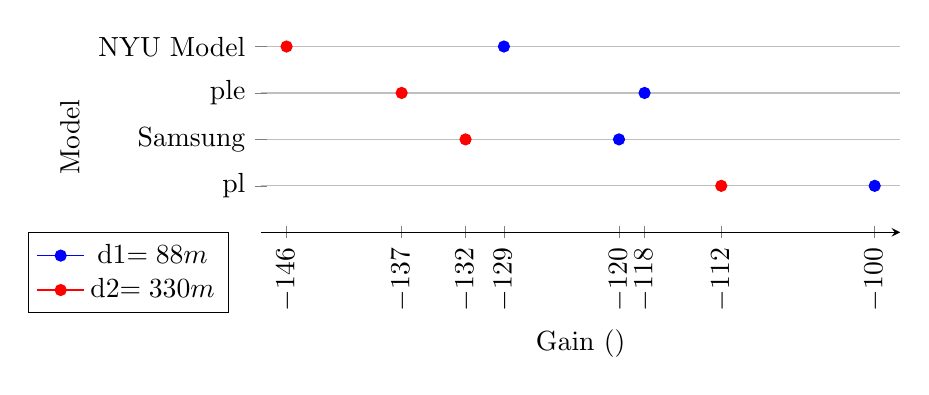
\begin{tikzpicture}
		\begin{axis}
			[
				axis x line=bottom,
				axis y line=left,y axis line style={draw=none},
				ymajorgrids=true,
				xmin=-148,xmax=-98,
				ymin=0,ymax=4.1,
				ytick={1,2,3,4}, yticklabels={\ac{pl}, Samsung, \ac{ple}, NYU Model},
				xtick={-146,-137,-132,-129,-120,-118,-112,-100},
				xticklabel style={rotate=90},
				xlabel=Gain (\si{\decibel}),
				ylabel=Model,
				height=4cm,
				width=0.8\linewidth,
				legend style={at={(-0.05,0)},anchor=north east}
			]
			%PLd1
			\addplot [mark=*,color=blue] coordinates {(-100,1)};
			\addlegendentry{d1$ = 88 m$}

			%PLd2
			\addplot [mark=*,color=red] coordinates {(-112,1)};
			\addlegendentry{d2$ = 330 m$}

			%Samsungd1
			\addplot [mark=*,color=blue] coordinates {(-120,2)};

			%Samsungd2
			\addplot [mark=*,color=red] coordinates {(-132,2)};

			%PLEd1
			\addplot [mark=*,color=blue] coordinates {(-118,3)};

			%PLEd2
			\addplot [mark=*,color=red] coordinates {(-137,3)};

			%NYUd1
			\addplot [mark=*,color=blue] coordinates {(-129,4)};

			%NYUd2
			\addplot [mark=*,color=red] coordinates {(-146,4)};

		\end{axis}
	\end{tikzpicture}
	\caption{Graph Comparing the PL Calculated by Various Channel Models}
	\label{fig:PLcomp}
\end{figure}

\par
One can see that free space propagation, modelled by \fref{eq:friis} and graphed as \ac{pl}, is by far the most optimistic of the models.
This is to be expected due to the simplifying assumptions it makes.

\par
Samsung's model \cite{khan:2011}, free space propagation with an additional \SI{20}{\decibel} loss, is comparable to \ac{ple} for the \ac{ccu} but is more optimistic than \ac{ple} for the \ac{ceu}.
It is interesting to note that an additional \SI{20}{\decibel} loss is still quite optimistic as compared to more complex models.

\par
We can see that the model shown in \fref{eq:nyu}, with the values described above, is more pessimistic than the other models.
It aligns with results found in \cite{akdeniz:2014}, which say measured results were about \SI{30}{\decibel} weaker than free space propagation.
Comparing the results of \fref{eq:nyu} to \fref{eq:ple} the relative loss of the \acp{ccu} is greater than that of the \acp{ceu}.

\par
I believe that the NYU model, detailed above, is a suitable model to use for the large scale fading going forward.
It is clear that Friis' Equation, and Samsung's adaption, are far too optimistic.
Though I believe that the values selected for \ac{ple} are well founded in the literature, I believe that the empirical model proposed by NYU will give harsher testing.
Harsher models can be seen as a worst case scenario and useful for testing the feasibility of \ac{noma} and results of tests and simulations.

\section{Basic NOMA Simulations}
\label{sec:basicsim}

\par
With the channel model chosen, per \fref{sec:ch}, rate simulations of \ac{noma} systems were conducted using \fref{eq:nomagen} to calculate the rate.
In these simulations the conditions were as follows:

\subsection{Channel Model}
\label{sec:bnsch}
The large scale fading of the channel model is as described in \fref{sec:ch}, this equates to the \ac{pl} of the signal and is largely dependent on distance and frequency.
To finalise the channel model small-scale fading was represented by summing random complex numbers to the \ac{pl} figure.
The small-scale fading has not much effect on the basic \ac{noma} case, as there is only one antenna on each \ac{ue} and the \ac{bs}, though it adds some variation to independent simulations.

\subsection{Distances}
\label{sec:distances}
In each simulation distances for each of the \acp{ue} are randomly generated, independent of each other, but were ultimately sorted by least to greatest.
The distances of the different \acp{ue} fell within the range of \SIrange{50}{250}{\metre}.
These distances were chosen to reflect a \ac{ccu} and a \ac{ue} at the likely edge of a \ac{mmwave} small cell network \cite{nguyen:2017}.

\subsection{Power Allocation}
The \ac{pa} for these early simulations was to run brute force calculations for each \ac{ue}.
This is to say that, particularly with a 2-\ac{ue} simulation the powers assigned can all be known and can all be computed.
This is not efficient but given the low degree of complexity inherent in these systems it is sufficient.

\subsection{2-UE Simulations}
\label{sec:s2ue}

\par
\Fref{fig:s2ueRate} is representative of the results found from basic \ac{noma} simulations, following the conditions outlined above.

\begin{figure}[htb]
	\centering
	\includegraphics[width=1\linewidth]{simple2ueNOMArate}
	\caption{2-UE NOMA Rate}
	\label{fig:s2ueRate}
\end{figure}

\par
It is clear to see that these simulations greatly favour the \ac{ccu}.
The rates achieved by the \ac{ceu} are low and the best sumrates are achieved by excluding that \ac{ue}.
These results are quite pessimistic and are not promising for the promise of \ac{noma} generally.

\par
The results seen in \fref{fig:s2ueRate} are indicative of \ac{ue}\tsb{1} benefiting from good \ac{sic} while \ac{ue}\tsb{2} suffering from interference.
It is clear, therefore, that more successful results would require better \ac{pa} to the \ac{ceu} for the relative ratio of distances.
Alternatively, if the \ac{ceu} were closer to the cell centre losses across the channel would be lowered, perhaps improving throughput.

\section{Beamforming NOMA}
\label{sec:bfsim}
The conditions and assumptions for the \ac{bf} simulations were similar to those in \fref{sec:basicsim}.

\par
In the basic \ac{noma} simulations, small-scale fading added variability to the only channel between \ac{bs} and \ac{ue}.
The key difference for these simulations is that there are more antennas at the \ac{bs}.
This has two main effects:

\begin{itemize}
	\item
		The small-scale fading in the channel model now introduces variability for all channels between \ac{bs} antennas and a \ac{ue}.
	\item
		The throughput calculation now computes, for each set of powers, the throughput at different \acl{bf} nodes.
		This is equivalent to considering non-uniform radiation patterns that can be seen with \acl{bf} techniques.
\end{itemize}

\par
The addition of extra \ac{bs} antennas has the opportunity to increase the throughput of individual \acp{ue} and, by extension, the sumrate of the system.
Using many antennas allows transmissions to take on a directionality, as compared to isotropic transmission, though radiation patterns will still be imperfect.
This allows for more efficient use of power, increasing the power of the signal at a receiving \ac{ue}.
Another benefit of directionality, aside from increasing the power at the desired receiver, is the potential reduction in inter-\ac{ue} interference.
Reducing interference would benefit other \acp{ue} and as a result benefits the system throughput as a whole.
The benefits of \acl{bf}, of course, being derived from the relationship between \ac{sinr} and throughput.

\subsection{System Model}
\subsubsection{Notation and Equations}
The system comprises of a \ac{bs}, with 16 antennas ($N_{\mathrm{Tx}}$), and 2--8 \acp{ue} ($K$), the number of \acp{ue} stated when relevant.
The \ac{bs} uses \ac{noma} and \ac{bf} to communicate with the \acp{ue}.
The aim is to optimise the \acl{pa} while using a \ac{bf} algorithm to get the direction of the beam.

\par
The channel model is, as discussed above in sections \ref{sec:ch} and \ref{sec:bnsch}, based on \ac{pl}, given by \fref{eq:nyu}, and small scale fading, which also implies a directionality.
Let $ \mb{h}_k  \in \mathbb{C}^{N_{\textrm{Tx}}\times 1}$ be the channel for \ac{ue} $ k $.
Similarly, let $ \mb{w}_k \in \mathbb{C}^{1\times N_{\textrm{Tx}}}$ be the beamformer for \ac{ue} $ k $ which is given by

\begin{equation}
	\mb{w}_k = \sqrt{\beta_k} \mb{u}_k 
\end{equation}

\par
Where $\beta_k$ is the \ac{pa} for \ac{ue} $k$ and $\mb{u}_k \in \mathbb{C}^{1\times N_{\textrm{Tx}}}$ is the \ac{bf} direction, or the \ac{bf} precoder, for \ac{ue} $k$.
This will be determined by the \ac{bf} algorithm employed.

\par
The received signal at \ac{ue} $k$ is

\begin{equation}
	y_k = \sum_{j=1}^{k-1} \mb{w}_j \mb{h}_k + \mb{w}_k \mb{h}_k + \sum_{j=k+1}^K \mb{w}_j \mb{h}_k + n_k
\end{equation}

\par
Suppose that \ac{sic} is performed from \ac{ue} $K$ to \ac{ue} $k+1$.
The interference caused by \acp{ue} from $k+1$ is removed.
Thus, the \ac{sinr} at \ac{ue} $k$ is given by

\begin{align}
	\gamma_k 
	& = \frac{\left| \mb{w}_k \mb{h}_k \right|^2}{\sum_{j=1}^{k-1} \left| \mb{w}_j \mb{h}_k \right|^2 + N_0}
	= \frac{\left| \sqrt{\beta}_{k} \mb{u}_k \mb{h}_k \right|^2}{ \sum_{j=1}^{k-1} \left| \sqrt{\beta}_{j}\mb{u}_j \mb{h}_k \right|^2 + N_0} \\
	& = \frac{\beta_k \left|\mb{u}_k \mb{h}_k \right|^2}{\sum_{j=1}^{k-1} \beta_{j} \left| \mb{u}_j \mb{h}_k \right|^2 + N_0}
\end{align}

\par
The achievable rate of \ac{ue} $ k $ is given by

\vspace{-2em}

\begin{align}
	R_{k}(\bs{\beta}) 
	& = \log (1+\gamma_k) \\
	& = \log (1 + \frac{\beta_k \left|\mb{u}_k \mb{h}_k \right|^2}{\sum_{j=1}^{k-1} \beta_{j} \left| \mb{u}_j \mb{h}_k \right|^2 + N_0}) \label{eq:bfrate} \\
	& = \log ({\beta}_k \left| \mb{u}_k \mb{h}_k \right|^2 
	+ \sum_{j=1}^{k-1} \beta_{j} \left| \mb{u}_j \mb{h}_k \right|^2 + N_0)
	- \log(\sum_{j=1}^{k-1} \beta_{j} \left| \mb{u}_j \mb{h}_k \right|^2 + N_0) \label{eq:bfratelong}
\end{align}

\subsubsection{Simulation Parameters}
\label{sec:simpar}
The distances that are used as the variable inputs to \fref{eq:nyu} are randomly generated within the range of \SIrange{50}{250}{\metre}.
This follows the reasoning given in \fref{sec:distances}.
Keeping these conditions consistent allows for a more direct comparison between \ac{noma} with \ac{bf} versus Basic \ac{noma}.

\par
Before a transmission to the connected \acp{ue} the \ac{bs} ranks the \acp{ue} based on the norm of their effective channels, the norm of the 16 channel values.
Sorting \acp{ue} based on this norm sorts them from strongest to weakest, similar to \ac{ccu}--\ac{ceu}, allowing for \ac{sic} in a \ac{noma} system.
Ranking \acp{ue} like this is particularly important for scheduling in \ac{hnoma} and \ac{bf}-\ac{noma} schemes but simply used for \ac{sic} order otherwise.

\par
The problem of \ac{bf} for a \ac{noma} system can be decomposed into two parts:

\begin{itemize}
	\item Creating beams to target \acp{ue}
	\item \ac{uppa} or Scheduling and \ac{pa}
\end{itemize}

\par
These problems were approached independently, first testing the effectiveness of \ac{bf} in \ac{noma} systems before choosing a suitable \ac{bf} algorithm, and then finding a suitable means of \ac{uppa}.

\subsection{Random Beamforming}
\label{sec:rbf}
Random \ac{bf} was used to test the viability of \ac{bf} in this system.
Though it can be intensive to simulate a large set of random beams it can be indicative of an optimal result.
Therefore, comparing the resilts of random \ac{bf} with the brute force seach results from the basic \ac{noma} system in \fref{sec:basicsim}

\par
At this point \ac{pa} is still done by a \ac{bfs}.
Given that, and adding the complexity of using a brute force process to create random beams, it is only practicable to perform tests for systems with 2 or 3 \acp{ue}.
This shall be sufficient for the purpose of comparing to results from \fref{sec:basicsim}, as similar constraints limited the number of \acp{ue} there also.

\par
\Fref{eq:rbf} defines the random \ac{bf} precoder:

\begin{equation}
	\mb{u} = \textrm{rand}(1, N_{\textrm{Tx}})
	\label{eq:rbf}
\end{equation}

\par
Where $\textrm{rand}(x,y)$ creates a vector of random numbers with $x$ rows and $y$ columns.
Consequently, the beamformer for \ac{ue} $k$ is given by 

\begin{equation}
	\mb{w}_k = \sqrt{\beta_k} \enspace \textrm{rand}(1, N_{\textrm{Tx}})
\end{equation}

\par
A random vector is used here, in place of a traditional \ac{bf} algorithm, to test the feasibility of \ac{bf} generally.

\subsubsection{2-\acs{ue} Simulations}
\label{sec:rbf2ue}
Simulations of 2-\ac{ue} \ac{noma} systems, with systems characterised as above, yielded the following results.

\par
\Fref{fig:bf2ueRate} is representative of the most promising results of these 2-\ac{ue} \ac{bf} simulations.

\begin{figure}[htb]
	\centering
	\includegraphics[width=0.6\linewidth]{2UEmaxrate}
	\caption{2-UE BF NOMA Rate}
	\label{fig:bf2ueRate}
\end{figure}

\par
It is clear to see from \fref{fig:bf2ueRate} that the maximum sumrate of system is a rate which is non-exclusionary, unlike the results seen in \fref{sec:s2ue}.
Achieving maximum sumrate in the middle of the curve of achievable sumrates is noteworthy as it shows that \ac{noma} has the potential to improve spectral efficiency in absolute metrics.
This is to say that, in this simulation, \ac{noma} achieved a better rate by sharing the available spectrum than would have been possible if the spectrum were used by only one \ac{ue}.
Contrasting \fref{fig:bf2ueRate} with \fref{fig:s2ueRate} we can see that \ac{bf} made a noticeable improvement to the rate of the whole system, though a greater improvement to the rates seen by \acp{ceu}.

\subsubsection{3-NOMA Simulations}
\label{sec:rbf3ue}
For the 3-\ac{ue} \ac{bf} \ac{noma} simulations the conditions were the same as the 2-\ac{ue} equivalents.
A key difference with the 3-\ac{ue} case is that the \ac{pa} problem gets much more complicated, complexity grows with \acp{ue}.

\par
For some 3-\ac{ue} simulations the maximum rate was such that all three \acp{ue} had a respectable rate.
\Fref{fig:bf3ueRate} shows one such example.

\begin{figure}[htb]
	\centering
	\includegraphics[width=1\linewidth]{3UEmaxrateall}
	\caption{3-UE BF NOMA Rate --- Including All}
	\label{fig:bf3ueRate}
\end{figure}

\par
In the simulations ran the results in \fref{fig:bf3ueRate} were quite common.
However, another common result is that akin to what can be seen in \fref{fig:bf3ueRate2}, where one \ac{ue} would be excluded.

\begin{figure}[htb]
	\centering
	\includegraphics[width=1\linewidth]{3UEmaxrate12}
	\caption{3-UE BF NOMA Rate --- Including UE\tsb{1} and UE\tsb{2}}
	\label{fig:bf3ueRate2}
\end{figure}

\par
It is clearly ideal to have rates which permit more \acp{ue}, this is to say results more like those in \fref{fig:bf3ueRate} than in \fref{fig:bf3ueRate2}.
From examining the circumstances leading to these separate results it is clear that \ac{plr} is the key factor in how successful all three \acp{ue} will be.
Where in Basic \ac{noma} it may be preferable to choose two \acp{ue} with the greatest difference in channels  \cite{ding:2016}, this random \ac{bf} technique tended to favour \acp{ue} with similar \ac{pl}, to a point.
If two \acp{ue} were within $\sim$\SI{1}{\decibel} then typically the two \acp{ue} with the greatest \ac{pl} difference achieved the best rate, as was the case in \fref{fig:bf3ueRate2}.

\subsection{Beamforming Algorithms}
Given the success of random \ac{bf} seen in \fref{sec:rbf} we can see that there are measurable benefits to using \ac{bf} with \ac{noma}.
However, random \ac{bf} is not feasible in real systems as it is too resource intensive.
This leads us to consider some common \ac{bf} algorithms to generate the precoder, or to determine the direction of the beam.

\subsubsection{Zero Forcing Beamforming}
\ac{zf} is a \ac{bf} algorithm which aims to create nulls in the direction of other \acp{ue}, hence the name \acl{zf}.
\ac{zf} gives priority to reducing inter-\ac{ue} interference over maximising power in the direction of the desired \ac{ue}.
While this lowers the throughput of any one \ac{ue}, \ac{zf} \ac{bf} can be beneficial to the sumrate of the system as reduced interference boosts the throughput of other \acp{ue}.

\par
\Fref{eq:zf} defines the \ac{bf} precoder for \ac{zf} as:

\begin{equation}
	\mb{u} = \frac{\mb{H}^{\dagger}}{\lvert\lvert \mb{H} \rvert\rvert_{2}}
	\label{eq:zf}
\end{equation}

\par
Where $(\cdot)^\dagger$ denotes the pseudo-inverse operation, which is defined as $\mb{H}'(\mb{H}\mb{H}')^{-1}$, and $||\cdot||_2$ denotes the $\ell_{2}$-norm.
Consequently, the beamformer for \ac{ue} $k$ is given by

\begin{equation}
	\mb{w}_k = \sqrt{\beta_k} \frac{\mb{H}^{\dagger}}{\lvert\lvert \mb{H} \rvert\rvert_{2}}
	\label{eq:bfzf}
\end{equation}

\par
The pseudo-inverse operation, used in \ac{zf}, serves to create beams which create nulls in the directions of non-intended recipients of the signal.

\iffalse
\begin{figure}
	\centering
	\includegraphics[width=0.6\linewidth]{2ueZF}
	\caption{2-UE NOMA ZF BF}
	\label{fig:ZF}
\end{figure}
\fi

\subsubsection{Maximum Ratio Transmission Beamforming}
\ac{mrt} is a \ac{bf} algorithm which prioritises the maximisation of power in the direction of the desired \ac{ue} over the other factors, such as reducing inter-\ac{ue} interference.
This maximises the transmission power in the direction of the \ac{ue}, giving each \ac{ue} the best signal strength possible.

\par
The \ac{bf} precoder for \ac{mrt} is given by \fref{eq:mrt}:

\begin{equation}
	\mb{u_k} = \frac{\mb{h_k}^H}{\lvert\lvert \mb{h_k} \rvert\rvert_2}
	\label{eq:mrt}
\end{equation}

\par
Where $(\cdot)^H$ denotes the Hermitian operation and $||\cdot||_2$ denotes the $\ell_{2}$-norm.
Consequently, the beamformer for \ac{ue} $k$ is given by

\begin{equation}
	\mb{w}_k = \sqrt{\beta_k} \frac{\mb{h}_k^H}{||\mb{h}_k||_2} 
	\label{eq:bfmrt}
\end{equation}

\par
The Hermitian transpose, used in \ac{mrt}, serves to direct the beam in the direction of the \ac{ue}, as determined by \ac{csi}.

\iffalse
\begin{figure}
	\centering
	\includegraphics[width=0.6\linewidth]{2ueMRT}
	\caption{2-UE NOMA MRT BF}
	\label{fig:ZF}
\end{figure}
\fi

\subsubsection{ZF vs MRT}
Simulations of both \ac{zf} and \ac{mrt} were run, with \ac{noma} as the means of \ac{ma}, to determine the best \ac{bf} algorithm to use in a \ac{noma} system.
One may expect \ac{zf} to have superior performance due to the reduction of inter-\ac{ue} interference, or for \ac{mrt} to achieve better sumrates as \ac{sic} may be sufficient and higher signal strength may be a more important factor.
The simulations were necessary as it is not obvious which factors would lead to better system throughput overall.

\par
The maximum sumrates achieved using both \ac{zf} and \ac{mrt} are shown in \fref{tab:ZFvMRT}.
The numbers in this table pertain to the rate graph in \fref{fig:ZFvMRT}:

\begin{table}[htb]
	\centering
	\begin{minipage}{0.3\linewidth}
		\centering
		\captionsetup{width=0.8\linewidth}
		\captionof{table}{ZF and MRT Max Sumrates}
		\label{tab:ZFvMRT}
		\begin{tabular}{l r}
			\multirow{2}{*}{BF Method} & Sum Rate\\
			 & (bps/\si{\hertz})\\
			\hline
			MRT & 7.0\\
			ZF & 7.0\\
		\end{tabular}
	\end{minipage}
	\begin{minipage}{0.6\linewidth}
		\centering
		\includegraphics[width=0.9\linewidth]{2ueZFvMRT}
		\captionsetup{width=0.9\linewidth}
		\captionof{figure}{2-UE NOMA ZF BF vs MRT BF}
		\label{fig:ZFvMRT}
	\end{minipage}
\end{table}

\par
In \fref{fig:ZFvMRT} it is clear that the two \ac{bf} algorithms have comparable performance in this system on average.
However, it can be seen in the figure that \ac{mrt} is superior, by a slim margin, to \ac{zf} at all points along the sumrate curve.
Results in \fref{tab:ZFvMRT} don't quite reflect this as the results were closest at the optimal point on this curve and the precision is insufficient to show that here.

\par
Though the results were comparable, as \ac{mrt} achieved the best sumrates it is the \ac{bf} algorithm that will be used going forwards.
Therefore, the beamformmer from \fref{eq:bfmrt} is adopted as the beamformer for the rest of this thesis.

\subsection{User Pairing and Power Allocation for Beamforming NOMA}
\label{sec:uppabf}
Based on research presented above detailing \ac{noma} schemes and \ac{uppa} for \ac{noma}, the following schemes were considered as solutions to this aspect of \ac{bf} for \ac{noma}.

\begin{itemize}
	\item Brute Force Search
	\item An Iterative Algorithm
	\item \ac{hnoma}
	\item \ac{hnoma} with \ac{pf}
	\item \ac{noma} within \ac{bf} Beams
\end{itemize}

\subsubsection{Brute Force Search}
A \ac{bfs} is a very effective but inefficient way of finding the optimal \ac{pa} for a given system at a given time.
All possible \ac{pa} combinations are computed to find the solution which yields the greatest sumrate.
\Fref{eq:bfrate} equation is computed for each \ac{ue} for each set of \acp{pa} and then the rates are summed.

\par
Results from simulations of the \ac{bfs} approach can be seen in \fref{fig:nsc_bfs}

\begin{figure}[htb!]
	\centering
	\includegraphics[width=0.6\linewidth]{nsc_bfs}
	\caption{BFS NOMA Results}
	\label{fig:nsc_bfs}
\end{figure}

\par
It can be seen that adding more \acp{ue} to the \ac{noma} system increases the sumrate for $K$ \SIrange{2}{8}{}.
It is noticeable that the rate does not increase steadily.
Instead there are diminishing increases to sumrate for each additional \ac{ue}.
This is sensible as each \ac{ue} may put additional strain on the \ac{sinr} of other \acp{ue} and may not add much to the system throughput.

\subsubsection{Iterative Algorithm}
Though \ac{bfs} will find the optimal \ac{pa} for a given $K$-\ac{ue} systems, \ac{bfs} for \ac{pa} becomes too resource intensive to be practical when $K$ is relatively large.
An iterative algorithm may serve as a more efficient and equally effective solution to finding the best \ac{pa} for a set of \acp{ue}.
As the sumrate of a \ac{noma} system may be non-convex, the iterative algorithm will instead optimise a \ac{foa} of the equation for sumrate.

\iffalse 
\par
The \ac{foa} for a 2-\ac{ue} \ac{noma} system follows \fref{eq:foa2ue}.
For a $K$-\ac{ue} system it is given by \fref{eq:foagen} and follows these constraints:

\begin{equation*}
	\begin{aligned}
			\min \quad &\null f(x)\\
			\text{s.t.} \quad &\null A \cdot B \leq B, A_{eq} \cdot X = B_{eq} \\
			&\null C(X) \leq 0, C_{eq}(X) = 0\\
			&\null LB \leq X \leq UB
	\end{aligned}
\end{equation*}

\par
Where $A$ is a vector of $1$'s that is $K$ long and $B$ is the maximum transmission power of a tower.
\fi

\par
% 2-UE FIRST ORDER APPROXIMATION
\Fref{eq:foa2ue} is a \ac{foa} expansion of \fref{eq:bfratelong} for $K=2$.

\begin{equation}
	\begin{aligned}
		- & \quad \left[\log \left( \beta_1 \cdot \left|h_1 \cdot u_1 \right|^2 + N_0 \right)
		\vphantom{ \frac{\left| h_2 \cdot u_1 \right|^2}{\left| h_2 \cdot \beta_1^o \cdot u_1 \right|^2} }
		\right. \\
		& - \left[ \log \left(  N_0 \right) \right] \\
		& + \log \left( \beta_2 \cdot \left|h_2 \cdot u_2 \right|^2 + N_0 + \beta_1 \cdot \left|h_2 \cdot u_1 \right|^2 \right) \\
		& - \left. \left[ \log \left(  N_0 + \beta_1^o \cdot \left|h_2 \cdot u_1 \right|^2 \right)
		+ \frac{\left| h_2 \cdot u_1 \right|^2}{N_0 + \beta_1^o \cdot \left| h_2 \cdot u_1 \right|^2}
		\cdot \left(\beta_1 - \beta_1^o \right)
		\right]
		\right]
	\end{aligned}
	\label{eq:foa2ue}
\end{equation}

\par
\Fref{eq:foa2ue} is negative as the optimisation is a minimum.
By getting the minimum of the negative equation we are in fact finding the \ac{pa} which maximises the sumrate of the system.

\par
To test the iterative algorithm \ac{pa} against a \ac{bfs} \ac{pa} for the same \ac{noma} system.
In \fref{fig:2ueOptVSearch} we can see that the iterative method can start with an all zero \ac{pa} and quickly iterate to the optimal \ac{pa}, achieving the maximum sumrate.
This shows, for a 2-\ac{ue} \ac{noma} system, that the iterative algorithm matches the performance of \ac{bfs}.
The difference however is that the iterative method is much less resource intensive, particularly for high precision of \ac{pa} or for systems with large numbers of \acp{ue}.

\begin{figure}[htb!]
	\centering
	\includegraphics[width=0.6\linewidth]{2ueOptVSearch}
	\caption{Finding 2-UE NOMA Rate by Minimisation or Search}
	\label{fig:2ueOptVSearch}
\end{figure}

\par
As the 2-\ac{ue} case was successful \fref{eq:bfratelong} was adapted for $K$ \acp{ue}.

% GENERALISED FIRST ORDER APPROXIMATION
\ac{foa} for $K$ \acp{ue}
\begin{equation}
	\begin{aligned}
		- \sum^K_{k=1}
		& \left[
			\vphantom{
			\frac{\sum^{k-1}_{j=1} \left| \mb{u}_j \mb{h}_k \right|^2}
			{\sum^{k-1}_{j=1} \beta^o_j \left| \mb{u}_j \mb{h}_k \right|^2 + N_0}
			}
			\log
			\left(
				\beta_k \left| \mb{u}_k \mb{h}_k \right|^2
				+ \sum^{k-1}_{j=1} \beta_j \left| \mb{u}_j \mb{h}_k \right|^2
				+ N_0
			\right) \right. \\
			-
			& \left(
				\vphantom{
				\frac{\sum^{k-1}_{j=1} \left| \mb{u}_j \mb{h}_k \right|^2}
				{\sum^{k-1}_{j=1} \beta^o_j \left| \mb{u}_j \mb{h}_k \right|^2 + N_0}
				}
				\log
				\left(
					\sum^{k-1}_{j=1} \beta^o_j \left| \mb{u}_j \mb{h}_k \right|^2
					+ N_0
				\right)
			\right.\\
			+ &\enspace \frac{\sum^{k-1}_{j=1} \left| \mb{u}_j \mb{h}_k \right|^2}
				{\sum^{k-1}_{j=1} \beta^o_j \left| \mb{u}_j \mb{h}_k \right|^2 + N_0} \\
			 \cdot & \left. \left.
			 \left(
				\sum^{k-1}_{j=1} \beta_j - \beta^o_j
			 \right)
		\vphantom{
		\frac{\sum^{k-1}_{j=1} \left| \mb{u}_j \mb{h}_k \right|^2}
		{\sum^{k-1}_{j=1} \beta^o_j \left| \mb{u}_j \mb{h}_k \right|^2 + N_0}
		}
		\right) \right]
	\end{aligned}
	\label{eq:foagen}
\end{equation}

\par
\Fref{eq:foagen} is, like \fref{eq:foa2ue}, multiplied by $-1$ at the start at the optimisation is a minimisation.
As the 2-\ac{ue} equivalent in \fref{eq:foa2ue} was successful, a similar optimisation of \fref{eq:foagen} should also find the optimal result for higher values of $K$.
Results of simulations using this iterative method can be seen in \fref{fig:nsc}.

\begin{figure}[H]
	\centering
	\includegraphics[width=0.6\linewidth]{nsc_opt}
	\caption{Optimised NOMA Results}
	\label{fig:nsc_opt}
\end{figure}

\par
Comparing figures \ref{fig:nsc_bfs} and \ref{fig:nsc_opt}, or the same plots in \fref{fig:nsc}, one can see that the rates achieved using the iterative algorithm match the optimal results found using \ac{bfs}.
The benefit being the dramatic reduction in resources required to find the \ac{pa} for larger $K$ when using the iterative method.

\par
Though the theoretical sumrates demonstrated in figures \ref{fig:nsc_bfs} and \ref{fig:nsc_opt} are impressive with multiple \acp{ue} these rates may be worse in practice.
The main issues come with the complexity of the receivers in such a \ac{noma} system.
If there is an error during \ac{sic} error propagation will lead to a lot of resources spent decodign messages of other \acp{ue} to find the message was decoded erroneously.

\par
Similarly, even if \ac{sic} is carried out without errors the time required to decode many \acp{ue} messges would lower the actual throughput of any device, even though the theoretical throughput is high.

\par
Due to the potential issues with larger \ac{noma} systems other \ac{noma} schemes are considered in the rest of this section.
These schemes have achieve lower sumrates as the number of \acp{ue} increases but should be less susceptible to the issues, outlined above and elsewhere, that arise in larger \ac{noma} systems.

\subsubsection{Hybrid NOMA}
As is discussed in \fref{sec:hnoma} \ac{hnoma} blends traditional \ac{ma} techniques with \ac{noma} to reduce the complexity required to perform \ac{sic}.
Here \ac{hnoma} is used such that each orthogonal resource is accessed by no more than 2 \acp{ue}.
The number of resources groups, $M$, required can be described as a function of the number of \acp{ue}.
This is shown in \fref{eq:group}.

\begin{equation}
	M(K) = \floor*{K \div 2} + K\hspace{-0.7em}\mod{2}
	\label{eq:group}
\end{equation}

\par
For this implementation of \ac{hnoma} the resources are divided evenly between all $M$ groups.
The \acp{ue} are grouped based on their channel ranking.
As was discussed in \fref{sec:simpar}, the strongest un-grouped \ac{ue} is always paired with the weakest un-grouped \ac{ue}, as determined by the norm of their channel vectors captured as \ac{csi}.

\par
Due to the success of the iterative method it is used to determine the \ac{pa} of each group in instead of using \ac{bfs}.
As each group has full access to all resources, the 2-\ac{ue} \ac{foa} described in \fref{eq:foa2ue} is used.

\par
The results of simulations with the described \ac{hnoma} system can be seen in \fref{fig:nsc_h}.

\begin{figure}[H]
	\centering
	\includegraphics[width=0.6\linewidth]{nsc_h}
	\caption{H-NOMA Results}
	\label{fig:nsc_h}
\end{figure}

\par
\Fref{fig:nsc_h} shows that the sumrate increases within the set of even numbered \acp{ue}, where all groups have 2 \acp{ue}, and that the sumrate increases within the set of odd numbered \acp{ue}, where one group has 1 \ac{ue}.
However, for systems where there is a group with one \ac{ue} the sumrate is lower than that of a system with one \ac{ue} less, where all groups are full.

\par
The sumrate for the system is the average sumrate achieved across all resource groups.
This would suggest that sumrate should remain relatively consistent as \acp{ue} are added to the system, but it was established earlier that \ac{noma} achieves better sumrates with higher numbers of \acp{ue} per resource.
This explains the decline in sumrate for systems where a resource is occupied by only one \ac{ue}.
Single \ac{ue} systems bring down the average as they are not taking advantage of the resources to the same extent.

\subsubsection{Hybrid NOMA with Proportional Fairness}
To combat the underutilisation of resources seen in \ac{hnoma} systems with \ac{pf} were investigated. Scheduling is the only difference between these approaches to \ac{hnoma}.
Rather than splitting the available resources evenly, as with \ac{hnoma} above, in a system using \ac{hnoma} with \ac{pf} the percentage of resources available to each group corresponds to the relative strength of each resource group.
Group strength can be taken as the inverse of the cost of any one group gaining access to the medium, which correlates to the norm of the channel vectors for \acp{ue} within a resource group.
This can be described by $w_i = \frac{1}{c_i}$ where the weight $w_i$ is equal to the inverse of the cost $c_i$ of letting group $i$ gain access.

\par
The norm of the strongest \ac{ue} in a group was used as the weight that dictates the proportion of the resource they had access to, as the channel norm already has an inverse relationship with cost.
The strongest \ac{ue} in a group was used as to use the sum of the channel norms would give more weight to groups where the respective \acp{ue} had similar channel strengths.
Giving preference to these groups is not desirable as they tend to perform worse than groups with greater differences in channel norm.
The sum of all weights was normalised such that the resource was fully utilised.

\par
\Fref{fig:nsc_ph} shows results from simulations with the described \ac{pf} \ac{hnoma} system.

\begin{figure}[H]
	\centering
	\includegraphics[width=0.6\linewidth]{nsc_ph}
	\caption{H-NOMA with PF Results}
	\label{fig:nsc_ph}
\end{figure}

\par
By scheduling the \acp{ue} with \ac{pf} there should be a reduction in the sumrate drop caused single \ac{ue} groups as well as in the sumrate drop caused by generally weaker groups.
Ultimately, where \ac{hnoma} saw little benefit to sumrate by adding more \ac{ue} groups \ac{hnoma} with \ac{pf} should achieve a slight increase in sumrate when using larger numbers of \acp{ue}.
It can be seen comparing figures \ref{fig:nsc_h} and \ref{fig:nsc_ph}, or comparing the relevant series in \fref{fig:nsc}, that \ac{pf} \ac{hnoma} does achieve better results than \ac{hnoma} and that for greater numbers of \acp{ue} the effect of underutilised groups is largely mitigated.

\subsubsection{NOMA within Beamforming Beams}
\acf{bfnoma}, similar to \ac{hnoma}, aims to circumvent the issues with large numbers of \acp{ue} in a \ac{noma} system, 
This is done, as the name of this section suggests, by grouping \acp{ue} and targeting them within \ac{bf} beams then treating each beam as it's own \ac{noma} system.
Groups are formed of no more than 2 \acp{ue}, so \fref{eq:group} also describes the number of groups here.

\par
Unlike in \ac{hnoma} groups are not determined by channel strength but rather by the correlation between channels.
\acp{ue} are first sorted by the norm of their channel vector, then the strongest available channel is cross-correlated with the channels of the remaining \acp{ue} and is grouped with the most correlated \ac{ue}.
This is repeated for all \acp{ue}.

\par
By grouping \acp{ue} with higher channel cross-correlation it is easier to target those \acp{ue} with just one beam.
However, since the stronger \ac{ue} is the primary target of the beam the secondary \ac{ue} will likely achieve a lower throughput. 
Using one beam to communicate with a pair of \acp{ue} allows the \ac{bs} to treat each beam as its own \ac{noma} system, and therefore simplify \ac{sic} for all \acp{ue} when compared to a normal \ac{noma} wit \ac{bf}.

\par
Two approaches to \ac{bfnoma} were considered, both using the iterative method above:

\begin{itemize}
	\item Arbitrary \ac{pa}
	\item Constrained \ac{pa}
\end{itemize}

\par
The arbitrary \ac{pa} approach allows the iterative method to optimise the \ac{pa} for all \acp{ue} entirely arbitrarily.
The constrained \ac{pa} approach divides the available transmission power evenly between all resource groups, or beams.
Power is then allocated, using the iterative method, to the \acp{ue} in each beam based on the power allotted. 
Simulations showed the this worked better than arbitrary approach.
Arbitrary \ac{pa} should yield superior results with a \ac{bfs} but the aim of this investigation was to avoid such a means of \ac{pa}.

\par
The results of simulations with the described \ac{bfnoma} system can be seen in \fref{fig:nsc_bf}.

\begin{figure}[H]
	\centering
	\includegraphics[width=0.6\linewidth]{nsc_bf}
	\caption{BF-NOMA Results}
	\label{fig:nsc_bf}
\end{figure}

\par
The results shown in \fref{fig:nsc_bf} show a weaker, and almost inverted, pattern than that seen in the previous \ac{hnoma} results.
In fact, the 2-\ac{ue} \ac{bfnoma} system is the only one that fails to meet an average of $\sim$\SI{11.5}{bps\per\hertz}, which can be attributed to one \ac{ue}, per group, always having a less targeted beam.
The inter-\ac{ue} interference, and the way \ac{pa} was performed, hindered the sumrates across the board.
One can see that for odd numbers of \acp{ue} the results are generally superior.
This can be explained by beams with only one \ac{ue} experiencing less contention and interference.
Groups with with reduced interference would increase the sumrate overall, which contrasts with single \ac{ue} groups decreasing sumrate in \ac{hnoma} systems.

% GRAPHICAL COMPARISON
\subsection{Graphical Comparison}
\label{sec:graphcomp}
By examining the results from the \ac{noma} schemes explored in \fref{sec:uppabf} conclusions can be drawn about the effectiveness and efficiency of each relative to competing schemes.
\Fref{fig:nsc} shows a comparison of those results.
A tabular comparison of those results can be found in \fref{tab:nsc}.

\begin{figure}[H]
	\centering
	\includegraphics[width=\linewidth]{"NOMA Scheme Comparison"}
	\caption{NOMA Scheme Comparison}
	\label{fig:nsc}
\end{figure}

\par
From \fref{fig:nsc} it can be seen that the best sumrates were achieved by the \ac{bfs} method of \ac{pa} and that the iterative method matched it.
Of course, the iterative method achieved matching results in a fraction of the time taken by the \ac{bfs}, making it a superior method of \ac{pa}.
Though these schemes achieved high throughputs in simulations, the effects of potential \ac{sic} errors make other schemes more appealing for larger groups of \acp{ue}.

\par
It is clear that both \ac{hnoma} with \ac{pf} and \ac{hnoma} are the \ac{uppa} schemes which achieve the next best results, with the \ac{pf} variant showing better results.
\ac{pf} especially showed better results than round robin scheduling in systems with odd numbers of \acp{ue}.
\ac{hnoma} with \ac{pf} was able to perform better by compensating for systems which were yielding lower throughputs.
Both \ac{hnoma} schemes are underutilising the available resources, by design to reduce strain on \ac{sic}.

\par
\ac{bfnoma} was considered as a means of striking a balance between the simplicity of \ac{hnoma} and the throughput of full \ac{noma}.
Completely arbitrary \ac{pa} yielded very poor results, as the optimisation failed to find the global minimum but rather always found local minima which yielded low sumrates.
Constraining the \ac{pa} for the system did improve the throughput but it did not outperform \ac{hnoma} as desired.
This is a result of two significant disadvantages; poorly correlated \ac{ue} channels, and inter-beam interference.
These obstacles to \ac{bfnoma} proved too great for it to achieve sumrates comparable to any of the other schemes.

